% This file was created by matlab2tikz.
% Minimal pgfplots version: 1.3
%
%The latest updates can be retrieved from
%  http://www.mathworks.com/matlabcentral/fileexchange/22022-matlab2tikz
%where you can also make suggestions and rate matlab2tikz.
%
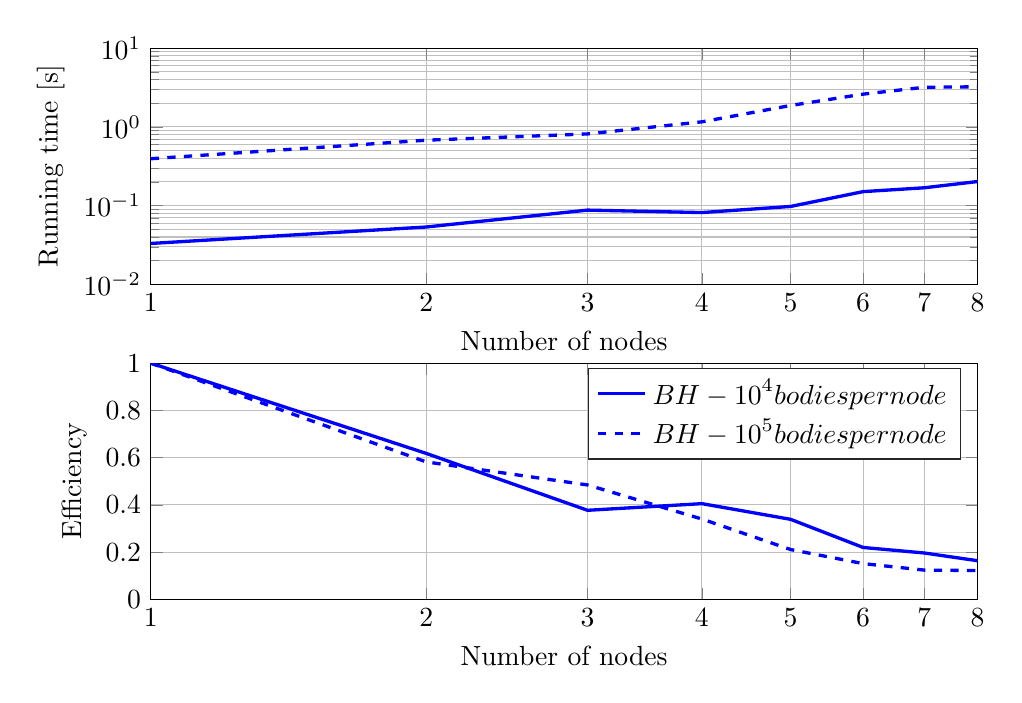
\begin{tikzpicture}

\begin{axis}[%
width=10.5cm,
height=3cm,
at={(0.758333in,5.37cm)},
scale only axis,
xmode=log,
xmin=1,
xmax=8,
xminorticks=true,
xlabel={Number of nodes},
xmajorgrids,
xminorgrids,
xtick={1,2,3, 4, 5, 6, 7, 8},
xticklabels={{1},{2},{3},{4},{5},{6},{7},{8}},
ymode=log,
ymin=0.01,
ymax=10,
yminorticks=true,
ylabel={Running time [s]},
ymajorgrids,
yminorgrids
]
\addplot [color=blue,solid,line width=1.2pt,forget plot]
  table[row sep=crcr]{%
1	0.03308295392\\
2	0.0535573495098039\\
3	0.0877561541372549\\
4	0.0816696460392157\\
5	0.0976765590196078\\
6	0.150651544509804\\
7	0.168636937058824\\
8	0.202365228823529\\
};
\addplot [color=blue,dashed,line width=1.2pt,forget plot]
  table[row sep=crcr]{%
1	0.394341795484314\\
2	0.677898941568627\\
3	0.814232577647059\\
4	1.15994181019608\\
5	1.87087138627451\\
6	2.60626458431373\\
7	3.18709408627451\\
8	3.23189081568628\\
};
\end{axis}

\begin{axis}[%
width=10.5cm,
height=3cm,
at={(0.758333in,1.37cm)},
scale only axis,
xmode=log,
xmin=1,
xmax=8,
xtick={1,2,3, 4, 5, 6, 7, 8},
xticklabels={{1},{2},{3},{4},{5},{6},{7},{8}},
xminorticks=true,
xlabel={Number of nodes},
xmajorgrids,
xminorgrids,
ymin=0,
ymax=1,
ylabel={Efficiency},
ymajorgrids,
legend style={legend cell align=left,align=left,draw=white!15!black}
]
\addplot [color=blue,solid,line width=1.2pt]
  table[row sep=crcr]{%
1	1\\
2	0.617710813227306\\
3	0.376987280780977\\
4	0.405082616669043\\
5	0.338699010817517\\
6	0.219599168582351\\
7	0.19617857449854\\
8	0.163481414827691\\
};
\addlegendentry{$\text{BH - 10}^\text{4}\text{ bodies per node}$};

\addplot [color=blue,dashed,line width=1.2pt]
  table[row sep=crcr]{%
1	1\\
2	0.581711773397705\\
3	0.484311001930025\\
4	0.339966877664021\\
5	0.210779745939442\\
6	0.15130535781276\\
7	0.123730829655321\\
8	0.122015816119264\\
};
\addlegendentry{$\text{BH- 10}^\text{5}\text{ bodies per node}$};

\end{axis}
\end{tikzpicture}%